% Possíveis TODO
% - expandir nas equacoes xx yy
\documentclass[a4paper,titlepage]{article}
\usepackage[utf8]{inputenc}
\usepackage[T1]{fontenc}
\usepackage[portuges]{babel}
% setspace - \doublespace \onehalfspace
% fullpage - ??
\usepackage{verbatim}
\usepackage{url}
\usepackage{hyperref}
\usepackage{graphicx}
\usepackage[bf]{subfigure}
\usepackage[bf]{caption}
\usepackage{amsmath,amssymb}
\usepackage{algorithm,algorithmic}
\usepackage{mathtools,empheq}
\usepackage{macrosfabbri-basic}
\usepackage{xcolor}

% ------------------------------------------------------------------------------
% Paper draft Comments and TODO's
%
% You have two versions of the macro
% \draftnote{My note}. The first version puts notes (e.g. My note in the example)
% into the margin of your document. The second formats the note as nothing. You
% 'comment out' the version of the macro you don't want (using a % at the
% beginning of the line).
\newcommand{\draftnote}[1]{\marginpar{\tiny\raggedright\textsf{\textcolor{blue}{\hspace{0pt}#1}}}}
%\newcommand{\draftnote}[1]{}
%
% This one is just for the comments for in-line text.
\newcommand{\indraftnote}[1]{\textcolor{blue}{\texttt{\footnotesize [#1]}}}
\newcommand{\todo}[1]{\indraftnote{todo: #1}} % Este  "a fazer" é para eu não esquecer



\begin{document}

\begin{titlepage}
\renewcommand{\title}{%
  {\LARGE Revis�o Comentada de Artigo}\\
  \mbox{Barycentric Subspace Analysis on Manifolds}%
}
\renewcommand{\author}{Nome Sobrenome}
\renewcommand{\date}{\today}
\newcommand{\info}{%
  \raisebox{4pt}[-4pt]{%
  
\includegraphics[height=1.3cm]{figs/logo-iprj.png} 
  \hspace{0.1in}
  }\\

  Instituto Polit�cnico -- IPRJ\\
  Universidade do Estado do Rio de Janeiro\\[2em]
  
  
\includegraphics[height=1.3cm]{figs/logo-ppgmc.png}\\
  Programa de P�s Gradua��o em Modelagem Computacional\\
  Disciplina de Variedades Diferenci�veis\\
  prof. Ricardo Fabbri\\[1em]

  Nova Friburgo, \date\\[1.5cm]
}

%% Abstand zwischen oberem Blattrand und Titel.
\newlength{\topToTitle} 
\setlength{\topToTitle}{0pt}

%% Abstand zwischen linkem Blattrand und Titel.
\newlength{\leftToTitle} 
\setlength{\leftToTitle}{-60pt}

%% Abstand zwischen Titel und Info-Feld.
\newlength{\titleToInfo} 
\setlength{\titleToInfo}{10cm}

%% \myTextWidth erhoehen, um Info-Feld weiter nach Rechts zu schieben.
\newlength{\myTextWidth}
\setlength{\myTextWidth}{\textwidth}
\advance\myTextWidth by 1cm


\thispagestyle{empty}
\vspace*{\topToTitle}
\begin{minipage}{\myTextWidth}
  \sffamily
  \hspace*{\leftToTitle}\begin{minipage}{11cm}
    \Large\textbf{Trabalho final}\\[1.5cm]
    \title\\[1.5cm]
    \author
  \end{minipage}\\

  %% \enlargethispage{} um ggfs. Titel und Info-Feld weiter
  %% auseinanderziehen zu koennen.
  \vspace*{\titleToInfo}

  \begin{minipage}{\textwidth}
    \flushright
    \info
  \end{minipage}
\end{minipage}%
\end{titlepage}


\section{Preliminares}

Este trabalho consiste em expandir o artigo de Paolo Zaini~\textit{et~al.}
intitulado ''\textit{Parameters estimate of Riemannian Gaussian distribution in
the manifold of covariance matrices.}``~\cite{zanini:hal-01325055},
cuja primeira página está reproduzida na Figura~\ref{fig:paper:page1}.
O presente texto é uma versão comentada do artigo,
expandindo o máximo possível os conceitos ligados a Variedades Diferenciáveis.
Desta forma, o presente texto é um superconjunto do referido artigo.
Ele contém todo o artigo, possivelmente em forma de recortes, com expansões e
comentários, e conexões com outros conceitos.

\begin{figure}
\centering
\frame{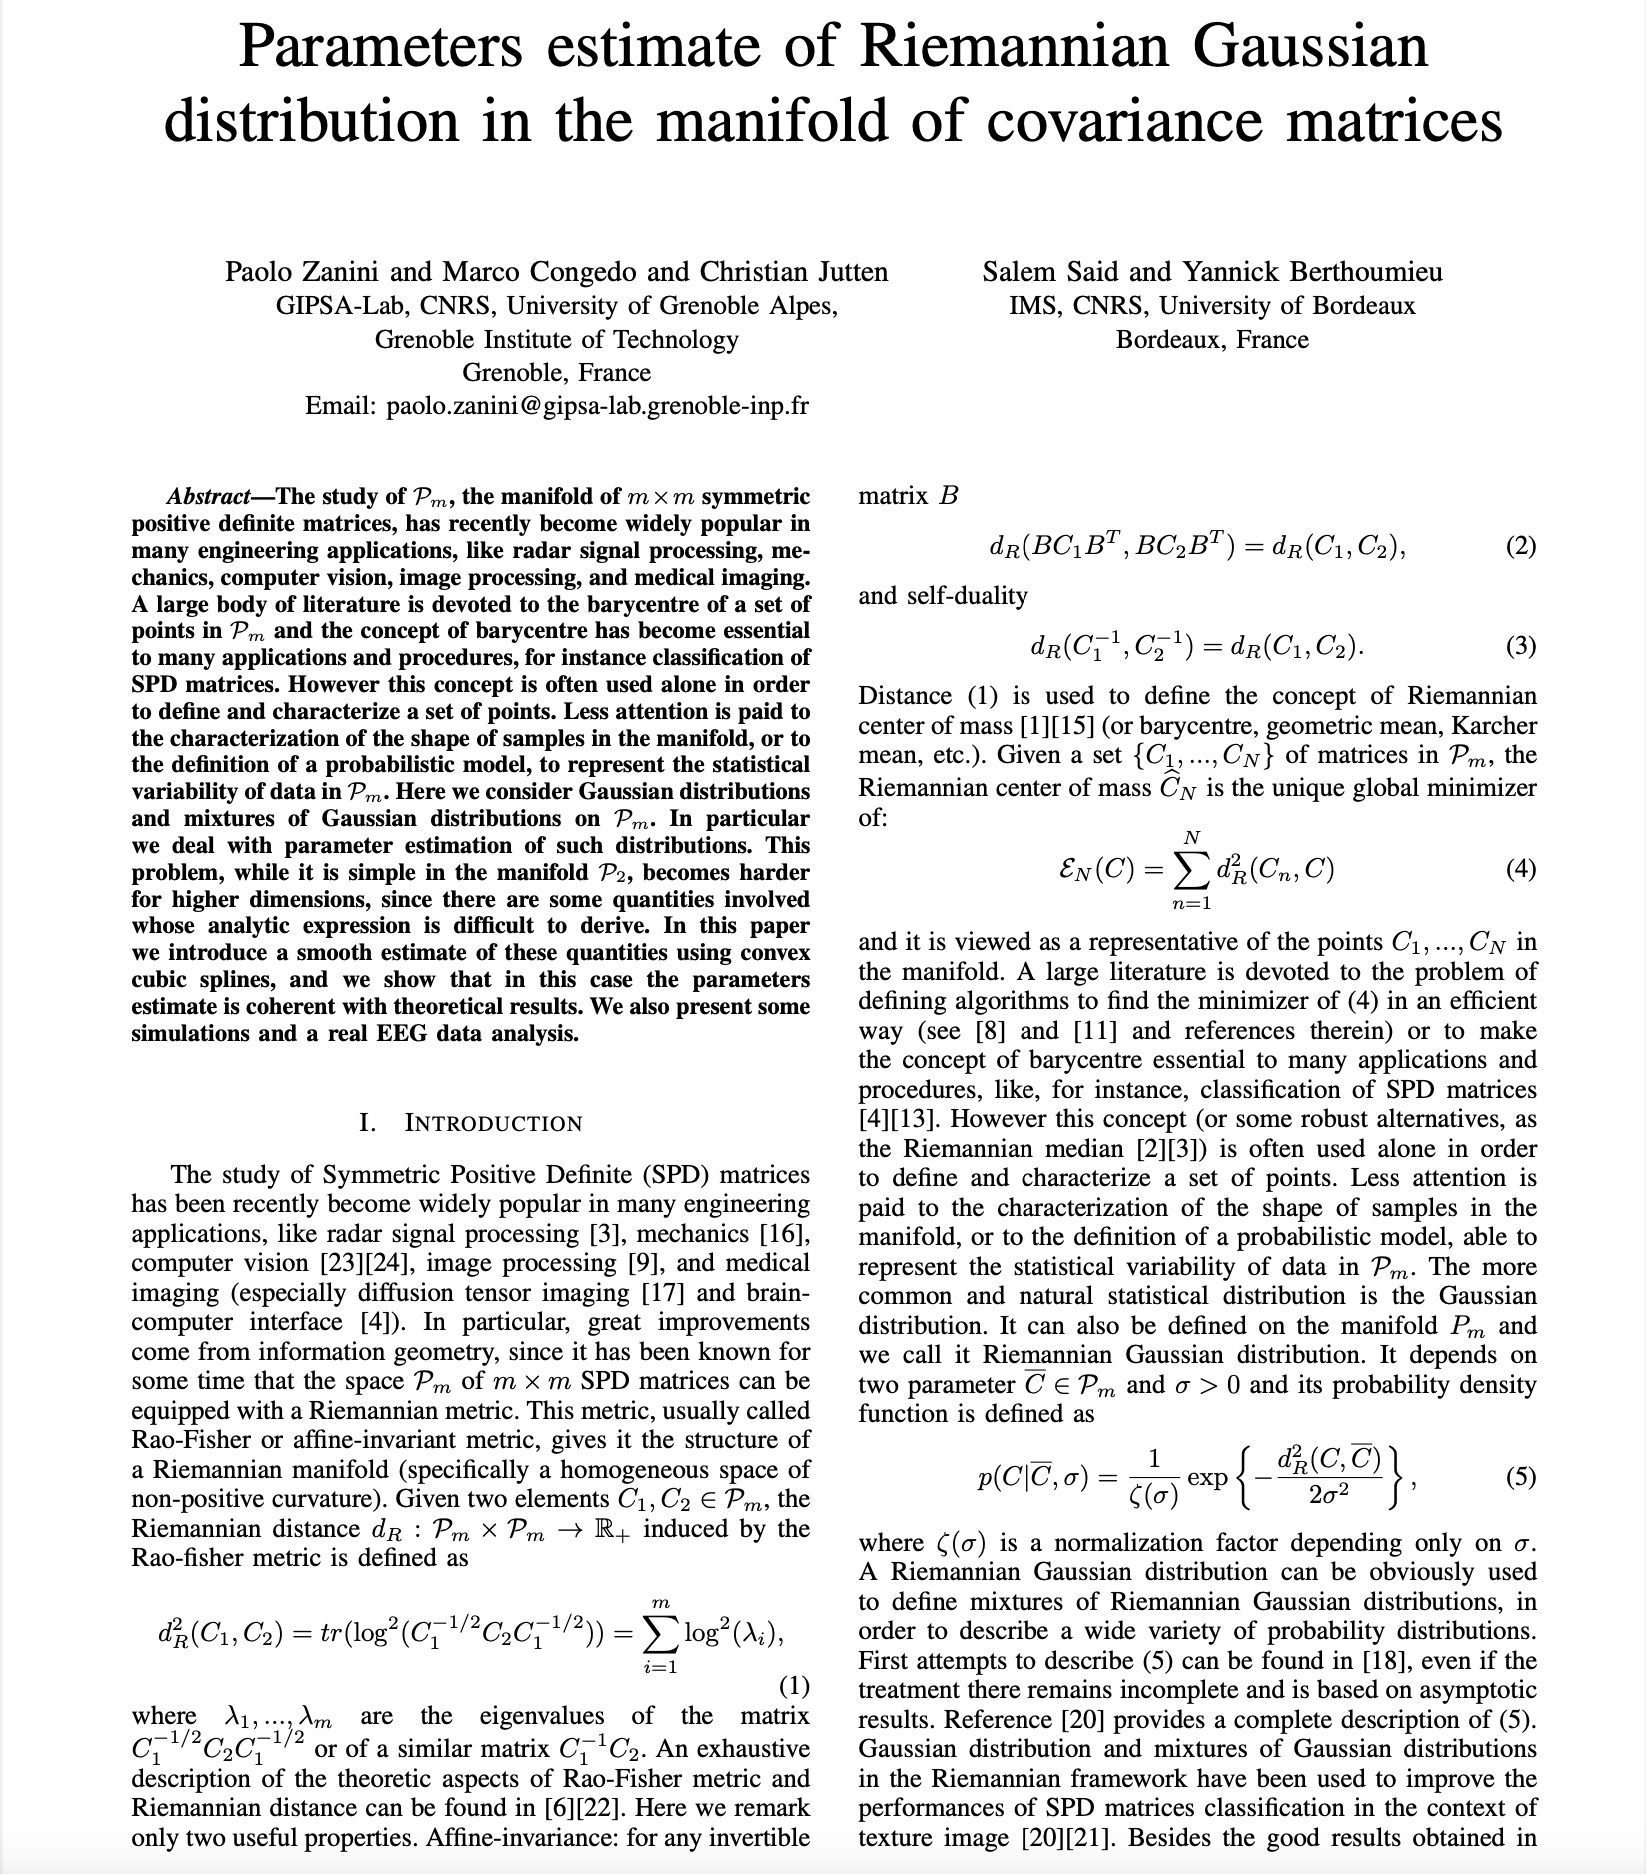
\includegraphics[width=.9\linewidth]{figs/page-01.png}}
\caption{% 
Primeira página do artigo sendo revisado. Acessível pela URL
\url{https://hal.inria.fr/hal-01325055}.
}\label{fig:paper:page1}
\end{figure}

Será utilizada uma mistura de línguas nesta revisão, sendo o inglês preferido
sempre que possível. Sendo assim, não teremos o trabalho de traduzir do inglês
algumas construções básicas do \LaTeX\ como \emph{Theorem} ou
\emph{Definition}.


\section{Tabela de Notação}

This section has a summary of the notation used in the paper.

\section{Commented and Expanded Abstract}

A figura a seguir mostra o \textit{Abstract} do paper. Os autores abordam o
estudo da variedade $\mathcal{P}_m$ das matrizes simétricas positivas-definidas
de dimensão $m \times m$. Este campo de pesquisa ultimamente tem se tornado
amplamente empregado em várias áreas da engenharia, como processamento de
sinais, visão computacional, processamento de imagens, valendo destacar a área
de imagiologia médica. Esta última é uma especialidade médica que se ocupa do
uso das tecnologias de imagem para realização de diagnósticos. As análises
realizadas neste trabalho utilizam dados simulados e dados reais de
Eletroencefalografia ou EEG, que é um método de monitoramento eletrofisiológico
utilizado para registrar a atividade elétrica do cérebro. 

\begin{center}
  \vspace{1em}
  \frame{\centering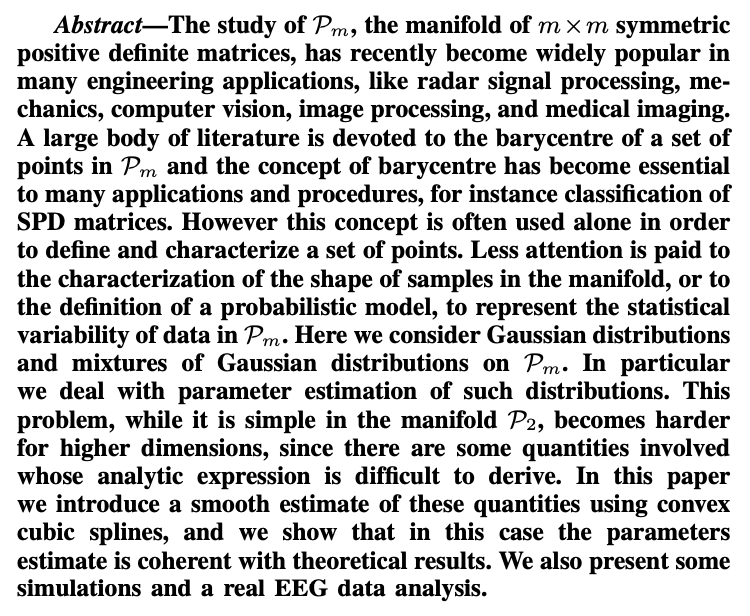
\includegraphics[width=0.8\linewidth]{figs/abstract.png}}
  \vspace{1em}
\end{center}


No contexto de álgebra linear, uma matriz positiva-definida (SPD, da sigla em
inglês \textit{Symmetric Positive Definite}) é análoga a um número real
positivo em muitos aspectos. Uma matriz simétrica $M$ com entradas reais é
positiva-definida se o número real $z^T M z$ é positivo para cada vetor coluna
real não-nulo $z$, onde $z^T$ é o seu
transposto~\cite{doi:PositiveDefiniteMatrices}.  Esta definição ainda pode ser
estendida para o domínio dos números complexos, no caso de matrizes
Hermitianas.

Os autores citam que grande parte da literatura está focada no estudo do
baricentro, ou centro de massa riemanniano, de um conjunto de pontos na
variedade de matrizes simétricas positivas-definidas $\mathcal{P}_m$.  O
conceito de baricentro é de notável importância para muitas aplicações, como a
classificação de SPD's. O problema do centro de massa riemanniano também é
conhecido na literatura como \textit{média riemanniana de
tensores}~\cite{moakher2005differential}.

Entretanto, os autores indagam que o conceito de baricentro tipicamente tem
sido utilizado apenas para a caracterização do conjunto de pontos. Não
obstante, pouca atenção tem sido empregada na caracterização da forma das
amostras na própria variedade ou ainda na definição do modelo probabilístico
que representa e governa a variabilidade estatística dos dados em
$\mathcal{P}_m$.

Neste trabalho, portanto, o problema de estimação de parâmetros de
distribuições Gaussianas em $\mathcal{P}_m$ será explorado para altas
dimensões, onde a tratabilidade do problema é mais difícil comparada ao caso
bidimensional.

\section{Commented and Expanded Section 1: Introduction}

\begin{center}
  \vspace{1em}
  \frame{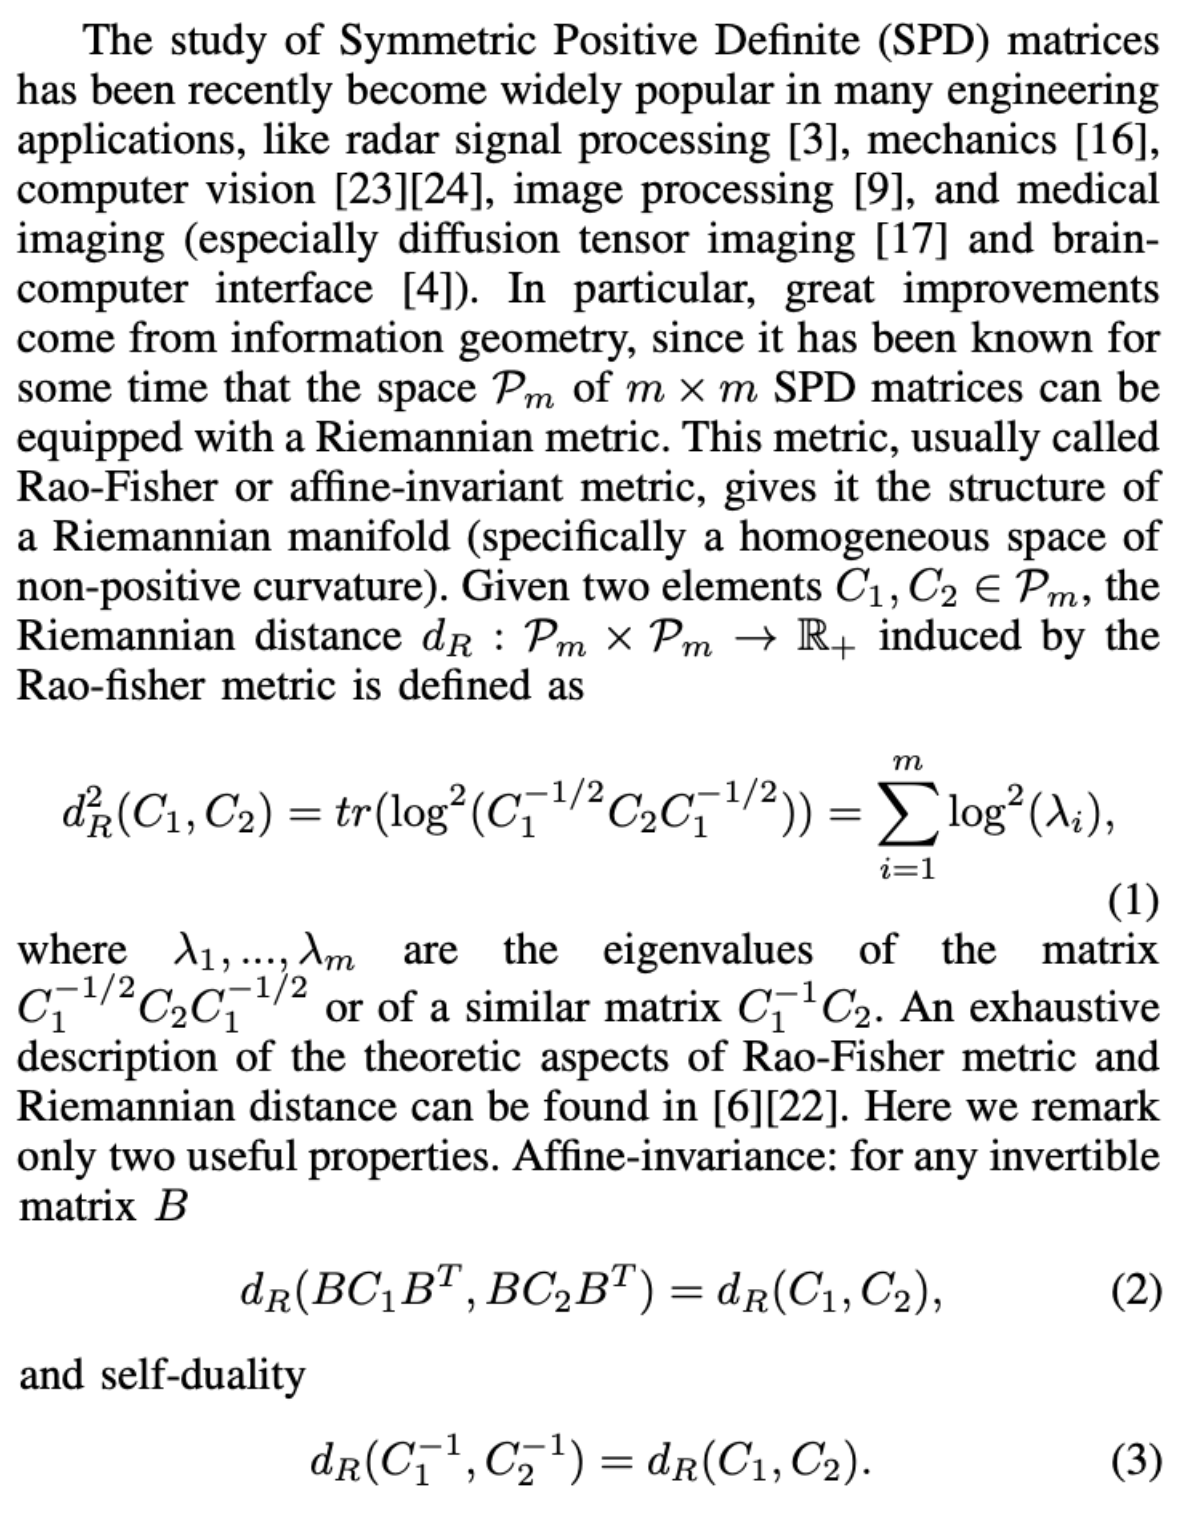
\includegraphics[width=0.8\linewidth]{figs/page-01-paragraph-01.png}}
  \vspace{1em}
\end{center}

A modelagem matemática do problema abordada pelos autores deriva os conceitos
da Geometria da Informação, área da matemática que utiliza ferramentas
geométricas no estudo de modelos estatísticos. Parte-se da variedade de
matrizes simétricas positivas-definidas $\mathcal{P}_m$ de dimensão $m \times
m$, sobre a qual define-se uma métrica Riemanniana. Introduzida em 1945 por
Rao, utilizando os fundamentos desenvolvidos por Ronald Fisher em 1921, esta
métrica tipicamente chamada de Rao-Fisher, define uma distância entre duas
distribuições de probabilidade, geodésicas, curvaturas e outras propriedades do
espaço~\cite{porto2013geometria}. Com esta métrica, definida pela Equação~(1),
a variedade adquire uma estrutura Riemanniana de um espaço homogêneo de
curvatura não-positiva.

Os autores destacam duas importantes propriedades da métrica de Rao-Fisher
$d_R^2 : \mathcal{P}_m \times \mathcal{P}_m \rightarrow \mathbb{R}_+$. A
primeira delas é a \textit{affine-invariance}, ou seja, a distância entre dois
elementos $C_1, C_2 \in \mathcal{P}_m$ não se altera o aplicar um conjunto de
transformações afins. A segunda propriedade é a \textit{self-duality}, onde a
distância entre $C_1^{-1}$ e $C_2^{-1}$ é a mesma que entre $C_1$ e $C_2$.  

\begin{center}
  \vspace{1em}
  \frame{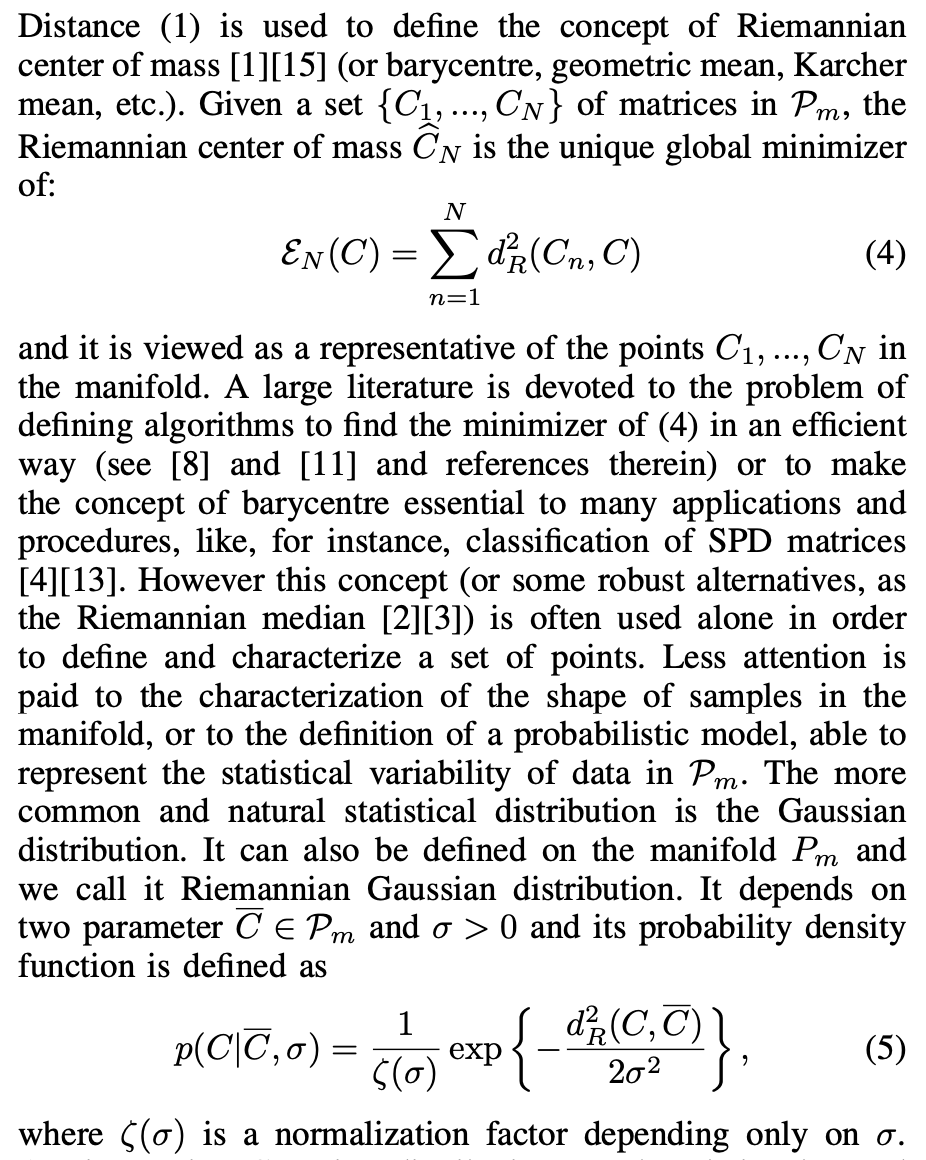
\includegraphics[width=0.8\linewidth]{figs/page-01-paragraph-02.png}}
  \vspace{1em}
\end{center}

A distância $d^2_R$ expressa pela Equação~(1), portanto, define o conceito de
centro de massa Riemanniano (ou baricentro, centro geométrico), o qual é utilizado
para a classificação de matizes SPD, dentre outras aplicações. Este centro de
massa, denotado por $\hat{C_N}$, é único e é dado pelo mínimo global da
Equação~(4). Várias técnicas tem sido empregadas para se encontrar este
minimizador. Como métodos de primeira ordem, pode-se citar o \textit{Steepest
Descent Method} e o \textit{Conjugate Gradient Method}. Também destacam-se
métodos de segunda ordem baseados na região de confiança (\textit{Trust region
method}) com suas variantes \textit{Exact Hessian}, \textit{Hessian by
decomposition}, \textit{Hessian by approximation} e ainda o
\textit{Broyden–Fletcher–Goldfarb–Shanno} (BFGS).

Entretanto, o conceito de centro de massa Riemannian tem sido amplamente
utilizado para definir e caracterizar um conjunto de pontos. Pouca atenção
tem-se dado para a caracterização da forma (ou \textit{shape}) das amostras na
própria variedade Riemanniana, o que possibilitaria caracterizar o modelo
probabilístico que governa os dados em $\mathcal{P}_m$.

Neste contexto de estatística, o modelo de distribuição de probabilidades
mais comum e naturalmente utilizado nas mais diversas áreas da ciência é o
modelo Gaussiano. Este modelo é dotado de particular notoriedade em virtude do
\textit{Teorema Central do Limite}, o qual estabelece que quando variáveis
aleatórias independentes são somadas, a distribuição de probabilidades
resultante tende a uma distribuição normal, ou
Gaussiana~\cite{fischer2010history}. Esta distribuição é parametrizada por
apenas duas quantidades, a média e a variância da variável aleatória.

Definido este modelo de distribuição de probabilidades na variedade
$\mathcal{P}_m$, tem-se então uma distribuição Gaussiana Riemanniana dada pela
Equação~(5), a qual depende da média $\bar{C} \in \mathcal{P}_m$ e da variância
$\sigma > 0$.

\begin{center}
  \vspace{1em}
  \frame{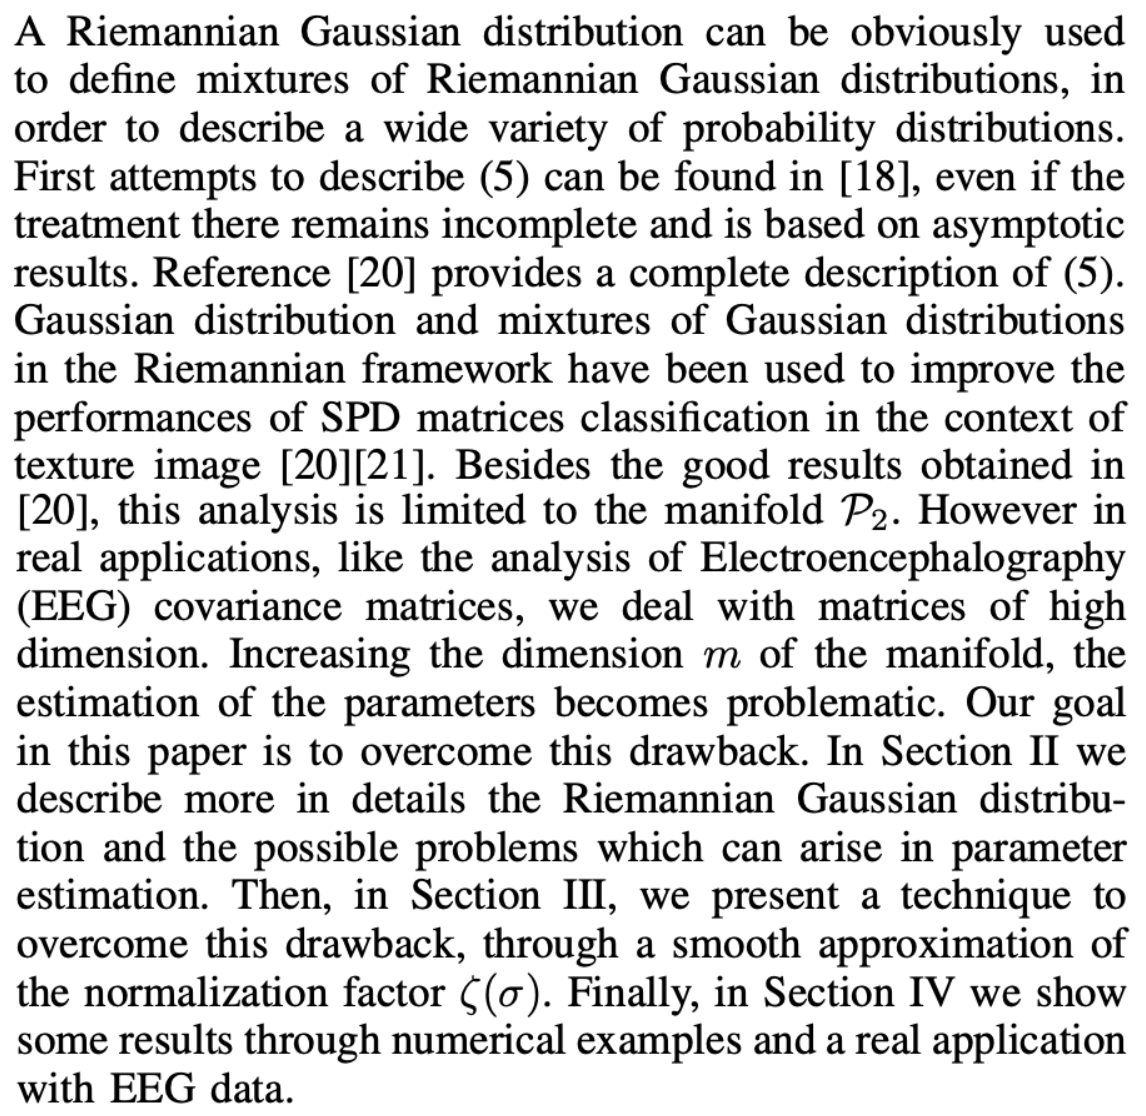
\includegraphics[width=0.8\linewidth]{figs/page-01-paragraph-03.png}}
  \vspace{1em}
\end{center}

O modelo de distribuição Gaussiana Riemanniana pode estendido para combinações
de distribuições Gaussianas Riemannianas, útil para descrever uma ampla
variedade de modelos probabilísticos. Estas construções tem sido utilizadas
para melhorar a performance de classificação de matrizes SPD no contexto de
imagens texturizadas, porém apesar dos bons resultados apresentados na
literatura, as análises até aqui tem se limitado em variedades de apenas duas
dimensões ($\mathcal{P}_2$). Contudo, para muitos outros problemas práticos,
como a análise de matrizes de covariância em Eletroencefalografia, lida-se com
fenômenos de alta dimensão onde o problema de estimação de parâmetros se torna
mais desafiador. Este trabalho se insere neste contexto, apresentando técnicas
para superar estas limitações.


\section{Commented and Expanded Section 2: Riemannian Gaussian Distribution}
Nesta seção os conceitos de Distribuição Gaussiana Riemanniana serão derivados
bem como os possíveis problemas que podem surgir na estimação de parâmetros.

\begin{center}
  \vspace{1em}
  \frame{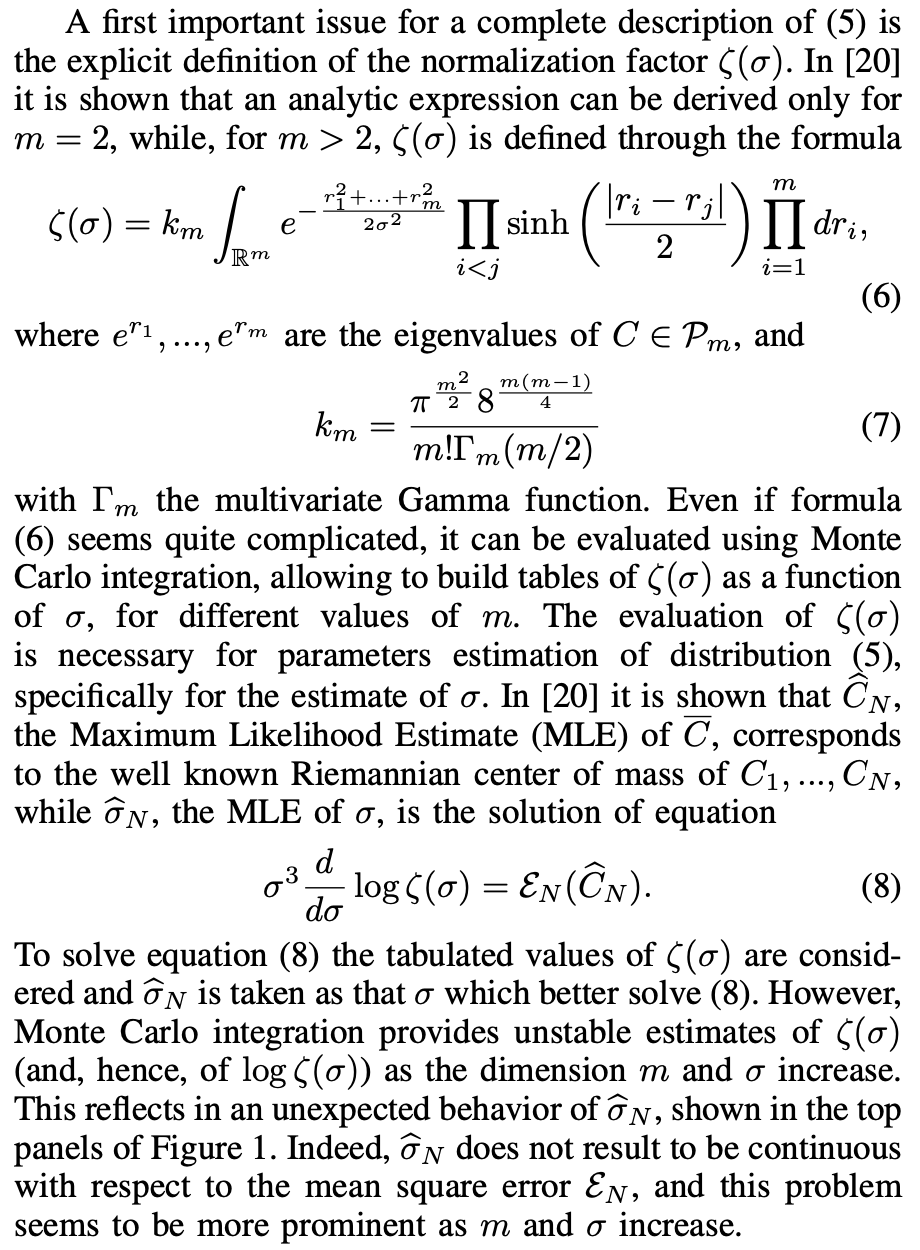
\includegraphics[width=0.8\linewidth]{figs/page-02-paragraph-01.png}}
  \vspace{1em}
\end{center}

\bibliographystyle{ieeetr}
\bibliography{refs}
%bib/edge-linking,bib/deformable,bib/medical,bib/graphics,bib/texture,bib/imaging,bib/tracking,bib/shape-papers,bib/bib-header,bib/video,bib/math-books,bib/math,bib/psych-books,bib/metric,bib/edge,bib/leymarie_pami_scaffold,bib/vision-books,bib/vision,bib/nn-search,bib/multidimscaling,bib/psychophysics,bib/indexing,bib/segmentation,bib/image-databases,bib/shape-matching,bib/neuro,bib/skeleton,bib/skeleton2D,bib/aspect-graphs,bib/recognition,bib/surface-networks,bib/ridge,bib/proceedings,bib/perceptual-grouping,bib/continuation,bib/graph-matching-2,bib/cooper}
%\input{paper.bbl}

% Assinaturas:
%\newpage
%\ \\\vspace{7cm}
%\center $\overline{\ \ \ Ricardo\ Fabbri\ \ \ }$
%\ \\\vspace{4cm}
%\center $\overline{\ \ \ Luciano\ da\ Fontoura\ Costa\ \ \ }$
\end{document}
